\documentclass[sigconf]{acmart}

\usepackage{hyperref}

\usepackage{endfloat}
\renewcommand{\efloatseparator}{\mbox{}} % no new page between figures

\usepackage{booktabs} % For formal tables

\settopmatter{printacmref=false} % Removes citation information below abstract
\renewcommand\footnotetextcopyrightpermission[1]{} % removes footnote with conference information in first column
\pagestyle{plain} % removes running headers

\begin{document}
\title{Big Data and Deep Learning}


\author{Jyothi Pranavi Devineni}
\affiliation{%
  \institution{Indiana University Bloomington}
  \city{Bloomington} 
  \state{Indiana} 
}
\email{jyodevin@umail.iu.edu}





\begin{abstract}
Big Data is providing new opportunities for various industries in different sectors to enhance their performance by performing analysis on the huge amounts of data available. However, this is not as easy as it is said. Storing, transforming and performing analysis on such large amounts of data requires good storing and computational power. Many solutions have been proposed to handle big data and use it to the benefit of the company like Map Reduce, Spark and so on. Deep learning is one of the popular branches of machine learning which plays a key role when it comes to big data analytics.
\end{abstract}

\keywords{Deep Learning, Big Data, Deep Belief Network, Convolutional Neural Network}
\maketitle
\section{Introduction}
Big data is the latest hot topic in the technical world and so is deep learning. Any data which consumes more than 1 Terra Bytes of memory is considered as big data. Social Media websites like Facebook generate more than 500 Terra Bytes  No conventional data base cannot store or manage more than 1 Terra Bytes of data. Hence, new technologies like Hadoop, Spark and so on have emerged to store and process large amounts of data. Hadoop used HDFS for storing the data and Map Reduce for processing the data. Scripting languages like Pig, Hive and Spark can also be used to process the data but, Map Reduce is a better option for processing unstructured data.

Deep Learning is another hot topic which is being discussed almost everywhere. Deep learning is one of the branches of machine learning, which uses machine learning techniques to solve the problems of data analysis and prediction. It does not follow any pre-defined algorithms, rather learns from the data. The learning can be supervised or unsupervised. Deep learning is used along with the systems with high computational power to address the big data problems. Many companies like Facebook, Apple, Google, Samsung are using the deep learning techniques to manage the huge amounts of data that is being generated daily by their search engines and websites. Not only this, deep learnig is also used in speech recognition, image processing, weather forecasting and so on. Hence, the voice assistants like Siri, Google home, Alexa make use of deep learning as well. As the data keeps getting huge, deep learning comes into play to process the data.

\section{Deep Learning}
Deep learning learns multiple levels of the deep architectures such as Deep Belief Networks(DBN), Convolutional Neural Networks(CNN) and so on. In this paper, a brief overview of DBN and CNN is given.

\subsection{Deep Belief Networks}
Any conventional neural network can only learn from the labelled data. But, most of the big data available is unlabelled. To take advantage of this massive amounts of unlabelled data, deep belief networks are used. They can not only learn from the labelled data, but also from the unlabelled data. They use both supervised and unsupervised learning techniques. It uses unsupervised techniques for pre- training and then to tune the data, it uses supervised techniques. Figure1 shows the architecture of DBN.



To achieve this, DBNs use Restricted Boltzmann Machines(RBMs). RBM consists of input layer, hidden layer and an output layer. Nodes in each layer are connected to all the nodes in the adjacent layer(input to hidden) and nodes in same layer are not connected to each other. Hence, we can say that nodes in same layer are independent of each other. The nodes in hidden layer are connected to the nodes in output layer according to the output to be generated. The network is pre-trained layer by layer using unlabelled data and the generative weights of each RBM are found using Gibbs sampling\cite{Hinton2006}. The output of an RBM is fed as input to the RBM in the next layer. This process is repeated until all the RBMs in a network are pre-trained. The weights represent the input data. Then, the output layer is constructed according to the required outputs. Then, fine tuning is performed using labels and by back propagation. RBMs can be trained on unlabelled and large amounts of data. The sampling probabilities of hidden and visible layers of an RBM with bernoulli distribution are as follows:

\begin{equation} p\left ( {h_{j}=1}\thinspace \vert \thinspace {\mathbf {v};W}\right ) =\sigma \left ( \sum \limits _{i=1}^I {w_{ij}v_{i}+a_{j}} \right )\end{equation}

\begin{equation} p\left ( {v_{i}=1}\thinspace \vert \thinspace {\mathbf {h};W}\right ) =\sigma \left ( \sum \limits _{j=1}^J {w_{ij}h_{j}+b_{i}} \right )\end{equation}

The weights are updated using the following equation. The $(t+1)^{th}$ weight is updated as:

\begin{equation} \Delta w_{ij}\left ( t+1 \right )=c\Delta w_{ij}\left ( t \right )+\alpha \left (\langle v_i h_j \rangle _{data}-\langle v_i h_j \rangle _{model} \right )\qquad\end{equation}

\subsection{Convolutional Neural Networks(CNN)}
CNN is another multi-layer neural network which is used for deep learning. CNN consists of multiple layers of convolution, activation and pooling. Figure2  depicts the architecture of a CNN


Convolution is a mathematical operation on two functions. It is defined by the following equation:

\begin{equation}
    s(t) = x(t)*w(t) = \sum^{\infty}_{a = -\infty}x(a)w(t-a)
\end{equation}

Convolution is used to extract the features from the input given to CNN, hence, it is called feature map stage. The output of convolution is called a feature map. The size of the feature map depends on three parameters:
\begin{enumerate}
    \item Depth
    \item Stride
    \item Zero-Padding
\end{enumerate}

Depth is the number of filters used for convolution. Stride is the number of pixels used to slide a filter across the input during convolution and appending zeros for the sake of convolution is called zero-padding.

After the convolution operation, activation function is applied to the output, to introduce non-linearity. Any non-linear activation function can be used for this purpose. 

After applying the activation function, the output is passed through pooling stage where different pooling operations such as average, sum, minimum, maximum, etc are applied. A window is defined and pooling is done in that window. The window slides over the input of the pooling stage by stride amount as discussed earlier.

After all these layers, a final layer is added using MLP for classifying the data or performing the regression, as per the required output. The steps followed in a CNN are, the filters and weights are randomly initialized first and then the data is passed through all the stages of CNN to get some output, then compare the actual and desired output and perform back propagation to update the weights accordingly.
\section{Deep Learning for  big Data}
Deep Learning is very useful for prediction, especially when it comes to unlabelled data. It has proved to be efficient in many applications. But, when it comes to big data, deep learning algorithms are not very efficient, as training the nodes requires iterative computing of the weights which is very difficult when the data is huge. Hence, parallel algorithms must be used for training deep architectures, when dealing with big data.

In 2012, Deng et al.\cite{Deng2012} proposed the concept of Deep Stacking Network(DSN) for parallel processing in deep architectures. Also there are other methods to address the big data problems, like improving the computation power, parallely computing the weights of hidden and visible layers, by distributing them across different machines and then integrating. It is nothing but a multi-node cluster in Hadoop. Each system is considered as a slave node computing the weights of a part of the hidden and visible neurons.

In addition to these techniques, systems with high computing power are used. One such example is GPU. Figure3 shows the architecture of a GPU:

The above GPU consists of four multi processors(MP), each MP consists of multiple streaming processors(SM) and each SM consists of multiple stream processors(SP). The stream processors share a common control logic and memory. The GPU also has a global memory. The architecture shown in the figure is a Single Instruction Multiple Thread architecture(SIMT). Such architecture is used when multiple computations are to be performed with less access time to the memory. The global memory in GPU is also a high-latency memory with high bandwidth. Here, the host represents the CPU. This architecture supports two levels of parallelism, namely memory level(MP) and thread level(SP). It facilitates multi-threading by running many hundreds of thousands of threads at a time.

\subsection{Deep Belief Networks for Big Data}
In deep learning architectures, millions of free parameters are considered to reduce the risk of over-fitting, in contrast to conventional architectures. For example Hinton and Salakhutdinov\cite{Hinton2006a} have used 3.8 million parameters for images and Ranzato and Szummer\cite{Ranzato2008} used three million parameters. But, the model proposed by Raina et al.\cite{2009} is far better than these models. Raina's model uses hundred million parameters for parallelizing the learning models which learn from unlabelled data, like DBNs.

Using GPU for parallelizing the DBN is not enough. Because, a considerable amount of time is wasted in transfering the data between the host and the global memories. Hence, to overcome this, a part of the training samples and the parameters are stored in the global memory itself while training. Also updating the parameters is done in GPU. In addition to memory and thread processing, data processing is also facilitated.

In DBNs, the weights are generated using Gibbs sampling using the same equations as for a non-parallel DBN, by generating sampling matrices P(x/h) and P(h/x) where the $(i,j)^{th}$ element is P($x_j$/$h_i$) in P(x/h) and p($h_j$/$x_i$) in P(h/x). Then, GPU is used to implement these two matrices. The weights are also updated in parallel using GPU.

\subsection{CNN for Big Data}
CNNs use GPUs for parallel processing to deal with big data. Both forward and backward propagation are used in training a CNN. Hence, both the propagations should be parallelized. To parallelize the forward propagation, each feature map in a CNN is assigned with some memory blocks, based on the size of the feature map and every thread in a block corresponds to a single neuron in a feature map. The CNN computations for each neuron in a map, such as convolution, applying activation function and pooling are performed in SP and the outputs are stored in the global memory.

In CNN, the weights are updated by back propagating the error. Back propagation can be parallelized by pushing or pulling the error signals. Although using GPUs facilitates parallel processing of data, it is only possible to process limited number of feature maps at any given time. For this purpose, Scherer et al\cite{2010} proposed an efficient method to use a circular buffer, which holds a small part of each feature map, loaded from global memory. Then, the threads parallely perform the convolution and the results are written back to the global memory. Krizhevsky et al.\cite{2012} proposed another yet faster method for processing big data using CNNs, by using two GPUs. Also, the speed of operation of CNN can be improved by using a ReLU or Rectified Linear Units activation function instead of any other activation functions.

\section{Deep Learning for High Volumes, Variety and Velocity of data}
The major concerns when dealing with big data are the volume of the data, variety of the data and velocity of the data. When dealing with large volumes of data, it is very difficult to train a deep learning algorithm using a single storage and CPU. Hence, distributed processing is preferred, which makes use of the multi-node cluster environment as in Hadoop. In such environment, the data and processing is distributed among different systems or nodes in the cluster for parallel processing and the outputs are again integrated at the master node.

Also, there are three types of data to be handled, structured, semi-structured and unstructured. Whatever the form the data might come in, it has to be stored and processed. There is not much difficulty in storing and processing structured data, but it is the semi-structured and un-structured data one faces a problem with. Also there is high velocity of data generated in many online site like the social media and so on, which needs to be accounted for in a timely manner. Deep learning can handle data of different varieties and with high velocity by using domain adaptation as discussed by Xue-Wen Chen and Xiaotong Lin.\cite{Chen2014}

\section{Conclusion}
This paper discusses two of the available deep learning architectures and how they are used to to address the big data problems. Deep learning has proved to be useful whenever one encounters big data. Deep learning architectures can be used along with systems which have high computation power and by performing parallel processing. 

\begin{acks}

  The authors would like to thank Professor Gregor Von Laszewski and all the associate instructors of the course I-523 for guiding us through.
\end{acks}


\bibliographystyle{ACM-Reference-Format}
\bibliography{report}

\begin{figure}[htp]
\centering
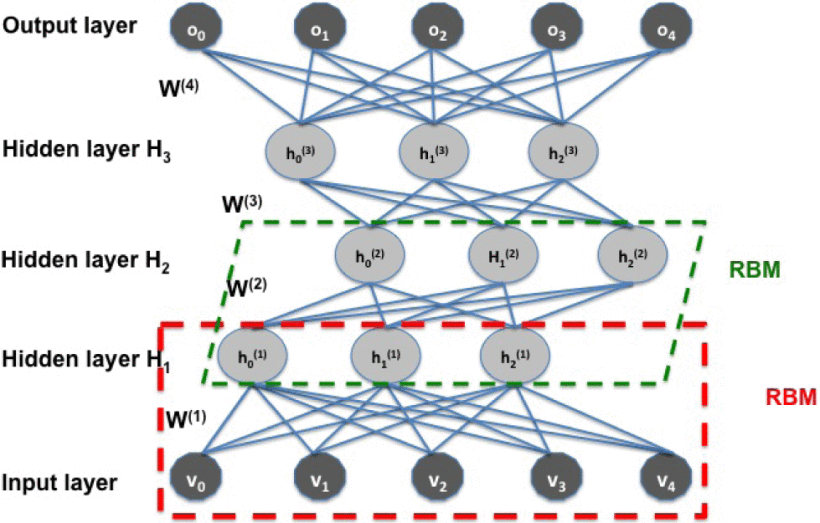
\includegraphics[width=80mm]{paper1-fig1.png}
\caption{DBN}
\label{fig:1}
\end{figure}

\begin{figure}[htp]
\centering
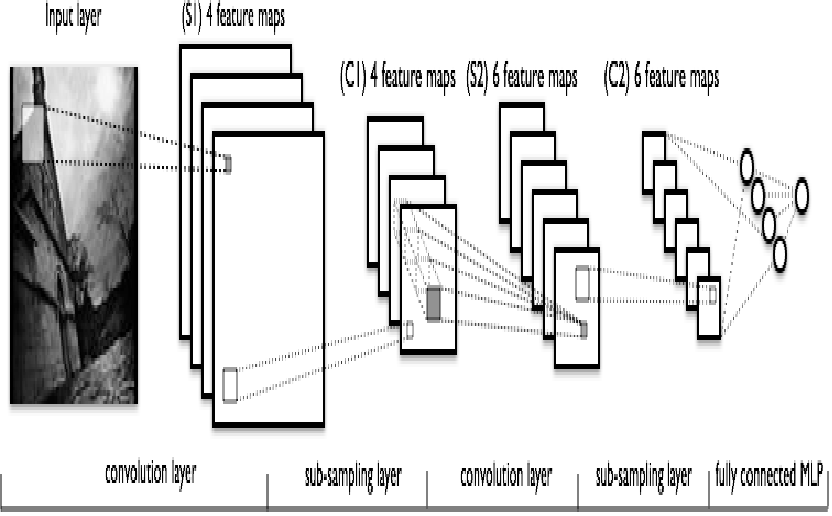
\includegraphics[width=80mm]{paper1-fig2.png}
\caption{CNN}
\label{fig:2}
\end{figure}

\begin{figure}[htp]
\centering
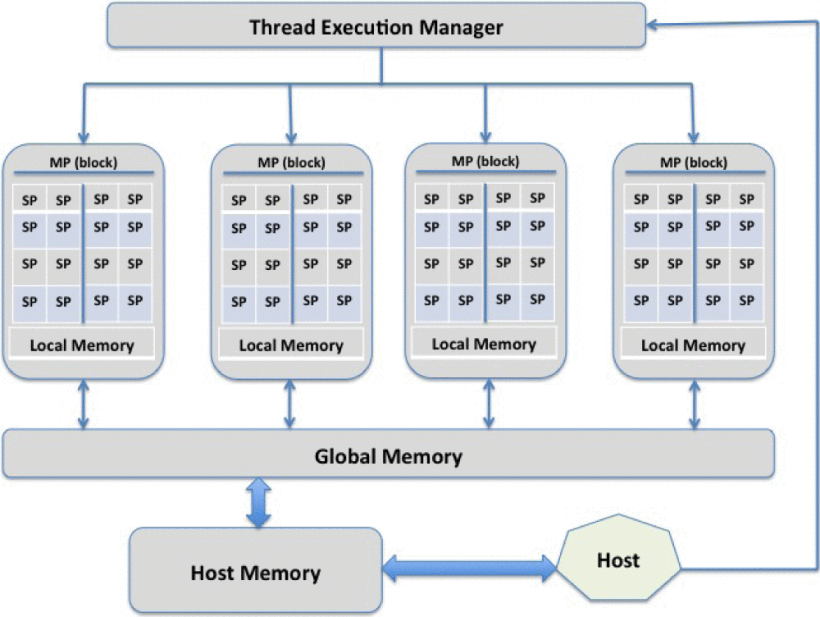
\includegraphics[width=80mm]{paper1-figure3.png}
\caption{GPU}
\label{fig:3}
\end{figure}

\end{document}
